% Evaluation
\chapter{Evaluation}\label{evaluation}
	In this section we report on our experimental results for the presented algorithms on three data sets of increasing size.
	Therefore, we first give insights on the data sets and how the network models are obtained. Afterwards we evaluate
	{\coverTree}s, \dijkstra, \astar (with $\asTheCrowFlies$), \alt, \csa and \multiModal methods such as the adopted \dijkstra
	and our simplified version of \anr on the given data sets.\\\\
	When evaluating shortest path queries on randomly chosen source and target nodes, the resulting paths tend to be long-range.
	However, in practice most queries are only local and algorithms like \dijkstra do not scale well with increasing range.
	To overcome this measurement problem, we introduce the notion of a \textit{Dijkstra rank} \libref{dijkstraRank}.
	\begin{mydef}\label{dijkstraRank}
		Given a graph $G = (V, E)$, the \textnormal{Dijkstra rank} of a node $v \in V$ is the number of the iteration in which,
		when running \dijkstra on the graph, it is polled from the priority queue (see \textbf{line 7} of \algoref{dijkstra}).
		
		That is the position $i$ for $v_i$ in the order of vertices when sorted ascending by their distance to the source, i.e.
		\begin{align*}
			v_1, v_2, \ldots, v_{|V|}
		\end{align*}
		with $\dist(v_i) \le \dist(v_{i + 1})$ for all $i$.
	\end{mydef}\quad\\
	Instead of choosing queries randomly, we only choose source nodes randomly and then select targets by their
	\textit{Dijkstra rank} to the source. Queries can then be sorted by the \textit{Dijkstra rank} and, by that,
	evaluated in terms of increasing range.

%Input data
\section{Input data}\label{inputData_sec}
	We consider three data sets, consisting of road and public transit data. The road network is extracted from \osm \libref{osm}
	formatted data and transit data is given in the \gtfs \libref{gtfs} format.\\\\
	Our data sets represent the region around the german cities \freiburgR and \stuttgartR. Their road network is
	of similar size, while our transit data for \freiburgR only includes tram data, whereas the data for \stuttgartR
	also includes train and bus connections. The size of our transit network for \stuttgartR is about ten times the size of
	the network for \freiburgR.
	
	Furthermore, we include a road and transit network for the country \switzerlandR. The transit data consists of train, tram and
	bus connections. Both networks are about three times the size of the {\stuttgartR}s.\\\\
	We obtain our road networks from \libref{freiburgRoadSource, stuttgartRoadSource, switzerlandRoadSource}
	and our transit networks from \libref{freiburgTransitSource, switzerlandTransitSource}.
	The transit data used for \stuttgartR is under restricted public access (refer to \libref{vvsContact}).

%OSM
\subsection{\osm}
	\osm \libref{osm} (OpenStreetMap) data is represented in a \xml structure describing
	\begin{itemize}
		\item[1.] \textit{nodes}, with an unique identifier and a coordinate given as pair of latitude and longitude;
		\item[2.] \textit{ways}, also with an unique identifier, consisting of multiple nodes referenced by their identifier;
		\item[3.] \textit{relations}, consisting of nodes, ways and other relations, representing relationships between the referenced data;
		\item[4.] \textit{tags} as key-value pairs, storing metadata about the other items.
	\end{itemize}
	\begin{lstlisting}[caption={\osm example data set, derived from \libref{osmExample}.},label={osmExample},style={XMLStyle},mathescape={true},
		float,floatplacement=ht]
<?xml version='1.0' encoding='UTF-8'?>
<osm version="0.6">
  <bounds minlon="7.253190" minlat="47.299090" maxlon="9.246965" maxlat="48.751520"/>
  <node id="29764598" lat="47.8512831" lon="7.9230269"/>
  <node id="669209525" lat="47.8513215" lon="7.9231227"/>
  <node id="3993821274" lat="47.8513342" lon="7.923183"/>
  <node id="832450227" lat="47.8157938" lon="8.8487527">
    <tag k="highway" v="motorway_junction"/>
    <tag k="name" v="Kreuz Hegau"/>
  </node>
  <node id="100036455" lat="47.5728421" lon="8.0365409">
    <tag k="name" v="Niederhof"/>
    <tag k="traffic_sign" v="city_limit"/>
  </node>
  <way id="29764598">
    <nd ref="669209525"/>
    <nd ref="3993821274"/>
    <tag k="highway" v="motorway"/>
    <tag k="oneway" v="yes"/>
  </way>
  <relation id="56688">
    <member type="node" ref="29764598" role=""/>
    <member type="node" ref="669209525" role=""/>
    <member type="way" ref="29764598" role=""/>
    <tag k="name" v="Bus line 1"/>
    <tag k="network" v="VVW"/>
    <tag k="ref" v="1"/>
    <tag k="route" v="bus"/>
    <tag k="type" v="route"/>
  </relation>
</osm>
	\end{lstlisting}\quad\\
	A small \osm example data set is shown by \lstref{osmExample}. Ways are used to represent roads consisting
	of nodes. Tags are used to describe metadata like speed limits for a road or whether it is a one-way street or not.
	However, the format also contains a lot of data not directly relevant for route planning, like shapes of buildings
	and outlines of public parks. Therefore, we filter \osm data and only keep relevant information.
	\begin{lstlisting}[caption={Tag filter for \osm ways.},label={osmFilter},style={FilterStyle},mathescape={true},
		float,floatplacement=ht]
--KEEP

#highways
highway=motorway
highway=trunk
highway=primary
highway=secondary
highway=tertiary
highway=residential
highway=living_street
highway=unclassified
highway=cycleway

#highwaylinks
highway=motorway_link
highway=trunk_link
highway=primary_link
highway=secondary_link
highway=tertiary_link
highway=residential_link

#non-standard
way=primary
way=seconday

--DROP

area=yes
train=yes
access=no
type=multipolygon
railway=platform
railway=station
highway=proposed
highway=construction
building=yes
building=train_station
	\end{lstlisting}\quad\\\\
	As we are only interested in the road network itself, we start by reading the ways. We filter them based on the tags
	described by \lstref{osmFilter}. Ways having at least one of the key-value pairs described under \textit{$--$KEEP}
	and none of the pairs under \textit{$--$DROP} are kept, as they represent roads of the network. All other ways are
	rejected, as well as all relations.
	After that, we read the nodes and only keep nodes that occurred at least once in any of the ways that passed the filter.
	Our road network is then build using the remaining nodes as graph nodes, translating the ways into edges between the nodes.
	
	Ways with a positive \textit{oneway} tag are translated into edges only going into the given direction, else we generate
	both edges for both directions. The cost of an edge is computed as the time it needs to travel the direct distance between
	the source and destination coordinates (see \defref{asTheCrowFlies}) with a certain speed. The speed is determined either
	by a given \textit{maxspeed} tag or the average speed for the road type defined by the \textit{highway} tag.
	Therefore, we use the average speed references shown by \tableref{highwaySpeeds}.
	\begin{table}[ht]
	 	\begin{center}
	 		\phantom{v}\quad\\
	 		\begin{tabular}{|l|r|}
	 			\hline
	 			\multicolumn{1}{|c|}{tag value}	&\multicolumn{1}{c|}{$\o$ km/h}\\\hline

				motorway		&$120$\\
				trunk			&$110$\\
				primary		&$100$\\
				secondary		&$80$\\
				tertiary		&$70$\\
				motorway\_link	&$50$\\
				trunk\_link		&$50$\\
				primary\_link		&$50$\\
				secondary\_link	&$50$\\
				residential		&$50$\\
				unclassified		&$40$\\
				unsurfaced		&$30$\\
				road			&$20$\\
				cycleway		&$14$\\
				living\_street		&$7$\\
				service		&$7$\\\hline
			\end{tabular}
		\end{center}
		\caption{Average speed in km/h for a \osm way with the corresponding value for the \textit{highway} tag.}
		\label{highwaySpeeds}
	\end{table}
	\begin{table}[ht]
	 	\begin{center}
	 		\phantom{v}\quad\\
			\begin{tabular}{|l||r|r|r|r|}
				\hline
							&\multicolumn{2}{c|}{data (MB)}	&\multicolumn{2}{c|}{Road graph}\\
							&\multicolumn{1}{c|}{raw}	&\multicolumn{1}{c|}{filtered}	&\multicolumn{1}{c|}{nodes}
								&\multicolumn{1}{c|}{edges}\\\hline
				\freiburgR		&$2\,260$	&$86$		&$743\,003$		&$1\,494\,883$\\
				\stuttgartR		&$2\,420$	&$118$	&$973\,142$		&$1\,950\,978$\\
				\switzerlandR	&$5\,530$	&$279$	&$2\,627\,645$	&$5\,226\,060$\\\hline
			\end{tabular}
		\end{center}
		\caption{Size of the \osm data sets, in megabyte (MB) before and after filtering, and the size of the resulting road graphs
			in amount of nodes $|V|$ and edges $|E|$.}
		\label{osmSize}
	\end{table}\quad\\\\
	The size of the resulting road graphs (see \sectionref{roadGraphSec}) for all three data sets is reported in \tableref{osmSize}.
	As seen, filtering the \osm data sets beforehand reduces the size of data that is to be processed by $95\%$ to $97\%$.
	The road graphs have approximately two edges per node. This is due to most streets being two-way streets, thus generating
	two edges per connection between two nodes. Obviously, road junctions are, compared to the amount of nodes, rare and thus,
	multiple edges do only rarely share the same node. The in- and outdegree of nodes is extremely low, mostly $2$ ($\approx 80\%$),
	as seen in \tableref{roadDegree}.
	\begin{table}[ht]
	 	\begin{center}
	 		\phantom{v}\quad\\
	 		\begin{tabular}{l}
			\begin{tabular}{|l||r|r|r|r|r|r|r|}
				\hline
							&\multicolumn{7}{c|}{indegree $\degG^{-}$}\\
							&\multicolumn{1}{c|}{0}	&\multicolumn{1}{c|}{1}	&\multicolumn{1}{c|}{2}	&\multicolumn{1}{c|}{3}
								&\multicolumn{1}{c|}{4}	&\multicolumn{1}{c|}{5}	&\multicolumn{1}{c|}{6}\\\hline
				\freiburgR		&$90$		&$64\,990$		&$611\,055$		&$59\,751$		&$7\,057$	&$58$		&$2$\\
				\stuttgartR		&$145$	&$109\,808$		&$759\,157$		&$93\,354$		&$10\,599$	&$76$		&$3$\\
				\switzerlandR	&$325$	&$235\,069$		&$2\,201\,945$	&$174\,333$		&$15\,767$	&$202$	&$4$\\\hline
			\end{tabular}\\
			\quad\\
			\quad\\
			\begin{tabular}{|l||r|r|r|r|r|r|r|r|}
				\hline
							&\multicolumn{8}{c|}{outdegree $\degG^{+}$}\\
							&\multicolumn{1}{c|}{0}	&\multicolumn{1}{c|}{1}	&\multicolumn{1}{c|}{2}	&\multicolumn{1}{c|}{3}
								&\multicolumn{1}{c|}{4}	&\multicolumn{1}{c|}{5}	&\multicolumn{1}{c|}{6}	&\multicolumn{1}{c|}{7}\\\hline
				\freiburgR		&$105$	&$65\,336$		&$610\,353$		&$60\,059$		&$7\,088$	&$60$		&$2$	&$0$\\
				\stuttgartR		&$162$	&$110\,002$		&$758\,740$		&$93\,545$		&$10\,607$	&$83$		&$3$	&$0$\\
				\switzerlandR	&$328$	&$235\,255$		&$2\,201\,711$	&$174\,247$		&$15\,884$	&$215$	&$4$	&$1$\\\hline
			\end{tabular}
			\end{tabular}
		\end{center}
		\caption{Table showing the number of nodes of the corresponding road graph that have a certain in- or outdegree.
		That is, the number of ingoing and outgoing edges respectively.}
		\label{roadDegree}
	\end{table}

%GTFS
\subsection{\gtfs}
	\gtfs \libref{gtfs} is short for General Transit Feed Specification, it defines a common format
	for public transit schedules. It comes compressed as \zip archive, consisting multiple
	text files formatted as \csv tables. The mandatory tables are
	\begin{itemize}
		\item[1.] \textit{agency.txt}, defining metadata about the transit agency;
		\item[2.] \textit{routes.txt}, containing information about complete routes, like all trips belonging to a bus line;
		\item[3.] \textit{trips.txt}, consisting of single trips, belonging to a route;
		\item[4.] \textit{stop\_times.txt}, having departure and arrival times at the stops for all connections in the network;
		\item[5.] \textit{stops.txt}, providing metadata and coordinates of all stops;
		\item[6.] \textit{calendar.txt} defining the service pattern at which routes are available.
	\end{itemize}
	Furthermore, there are a couple of optional tables of which we are only interested in
	\begin{itemize}
		\item[7.] \textit{transfer.txt}, provides transfer possibilities between stops and their duration.
	\end{itemize}
		\begin{lstlisting}[caption={\gtfs example data set, inspired by \libref{gtfsExample}.},label={gtfsExample},style={GTFSStyle},mathescape={true},
		float,floatplacement=ht]
// agency.txt
agency_id, agency_name, agency_url, agency_timezone, agency_phone, agency_lang
FunBus, The Fun Bus, , (310) 555-0222, en

// routes.txt
route_id, route_short_name, route_long_name, route_desc, route_type
A, 17, Mission, From lower Mission to Downtown., 3

// trips.txt
route_id, service_id, trip_id, trip_headsign, block_id
A, WE, AWE1, Downtown, 1
A, WE, AWE2, Downtown, 2

// stop_times.txt
trip_id, arrival_time, departure_time, stop_id, stop_sequence, pickup_type, drop_off_type
AWE1, 0:06:10, 0:06:10, S1, 1, 0, 0
AWE1, 0:06:20, 0:06:30, S3, 3, 0, 0
AWE1, 0:06:45, 0:06:45, S6, 5, 0, 0
AWD1, 0:06:10, 0:06:10, S1, 1, 0, 0
AWD1, 0:06:20, 0:06:20, S3, 3, 0, 0
AWD1, 0:06:45, 0:06:45, S6, 6, 0, 0

// stops.txt
stop_id, stop_name, stop_desc, stop_lat, stop_lon, stop_url, location_type, parent_station
S1, Mission St. & Silver Ave., , 37.728631, -122.431282, , ,
S3, Mission St. & 24th St., , 37.75223, -122.418581, , ,
S6, Mission St. & 15th St., , 37.766629, -122.419782, , ,

// calendar.txt
service_id, monday, tuesday, wednesday, thursday, friday, saturday, sunday, start_date, end_date
WE, 0, 0, 0, 0, 0, 1, 1, 20060701, 20060731
WD, 1, 1, 1, 1, 1, 0, 0, 20060701, 20060731

// transfers.txt
from_stop_id, to_stop_id, transfer_type, min_transfer_time
S3, S6, 2, 300
S6, S3 3, 180
	\end{lstlisting}\quad\\
	An example feed can be seen in \lstref{gtfsExample}. The format is similar to our definition of timetables (see \sectionref{timetable_sec}),
	with the difference that connections are not directly given as edges departing from one stop and another, but as pair of arrival and
	departure time at stops. Also, it contains a lot of metadata which we do not process.\\\\
	Construction of a realistic time expanded transit graph (see \defref{realisticTransitGraph}) is straightforward and mainly
	involves around parsing \textit{stop\_times.txt}. We build two nodes for every entry, one representing the arrival event at the stop
	and another for the departure. Furthermore, we create a transfer node for every arrival node, indicating a transfer at the given stop.
	Each arrival node is then connected by an edge with its corresponding departure and transfer node.
	
	After parsing all data, we connect departure nodes with the arrival nodes at the next stop in a trip. Therefore, we
	process each trip and follow the \textit{stop\_times.txt} entries belonging to that trip in the order defined by
	the \textit{stop\_sequence} field.
	
	As a next step, waiting edges are created by sorting transfer nodes of a stop ascending in time and then creating edges
	connecting them in that order. Finally, every departure node is connected to its previous transfer node. We find the
	transfer node by using a \textit{binary search} \libref{binarySearch} on the sorted list of transfer nodes for this stop.\\\\
	Timetables (see \defref{timetable}) are received similar. But simpler, as transfer nodes are not present. We process
	all stops and trips defined in \textit{stops.txt} and \textit{trips.txt} and obtain the sets $S$ and $T$ respectively.
	Connections are created by again processing entries in \textit{stop\_times.txt}, belonging to one trip, in the sequence
	defined by \textit{stop\_sequence}. We create one connection for every departure node with the corresponding
	next arrival node.
	
	For the footpaths, we initially take the transfers given in \textit{transfers.txt}. In order to increase the quality
	of our footpath model, we also connect stops with footpaths if they are within $600$ meters to each other.
	
	However, our footpaths need to fulfill strong properties (see \sectionref{timetable_sec}), which the given
	transfers usually not obey. Therefore, we have to add self-loop footpaths, if not present. And we need to compute
	the transitive closure of the given footpaths in order to ensure that they are transitively closed. Therefore, it is
	crucial that the range, for which close stops are connected, is kept low. Else, the amount of footpaths dramatically increases
	due to the transitive closure.
	
	The \textit{triangle inequality} property is ensured by rejecting given transfer durations and approximating all durations by using $\asTheCrowFlies$.
	Additionally, all footpath durations must not be lower than the transfer buffer used for the self-loop footpaths. We do so by taking the
	$\max$ of the transfer buffer and the calculated duration.
	\begin{table}[ht]
	 	\begin{center}
	 		\phantom{v}\quad\\
	 		\begin{tabular}{l}
			\begin{tabular}{|l||r|r|r|}
				\hline
							&\multicolumn{1}{c|}{data (KB)}	&\multicolumn{2}{c|}{Transit graph}\\
							&	&\multicolumn{1}{c|}{nodes}	&\multicolumn{1}{c|}{edges}\\\hline
				\freiburgR		&$1\,713$		&$613\,329$		&$1\,006\,862$\\
				\stuttgartR		&$32\,213$		&$4\,517\,511$	&$7\,415\,894$\\
				\switzerlandR	&$75\,477$		&$32\,688\,498$	&$53\,370\,236$\\\hline
			\end{tabular}\\
			\quad\\
			\begin{tabular}{|l||r|r|r|r|}
				\hline
							&\multicolumn{4}{c|}{Timetable}\\
							&\multicolumn{1}{c|}{stops}	&\multicolumn{1}{c|}{trips}
								&\multicolumn{1}{c|}{connections} &\multicolumn{1}{c|}{footpaths}\\\hline
				\freiburgR		&$713$	&$13\,249$		&$191\,194$		&$255\,495$\\
				\stuttgartR		&$7\,877$	&$90\,475$		&$1\,415\,362$	&$1\,926\,611$\\
				\switzerlandR	&$30\,227$	&$1\,014\,699$	&$9\,881\,467$	&$3\,793\,581$\\\hline
			\end{tabular}\\
			\quad\\
			\begin{tabular}{|l||r|r|r|r|}
				\hline
							&\multicolumn{4}{c|}{Footpaths}\\
							&\multicolumn{1}{c|}{given}	&\multicolumn{1}{c|}{self-loops}
								&\multicolumn{1}{c|}{close} &\multicolumn{1}{c|}{closure}\\\hline
				\freiburgR		&$0$		&$713$		&$9\,008$		&$245\,774$\\
				\stuttgartR		&$6\,080$	&$7\,877$		&$73\,730$		&$1\,838\,924$\\
				\switzerlandR	&$22\,402$	&$30\,227$		&$174\,698$		&$3\,566\,254$\\\hline
			\end{tabular}
			\end{tabular}
		\end{center}
		\caption{Size of the \gtfs feeds, in kilobyte (KB) and the size of the resulting realistic time expanded transit graphs
			in amount of nodes $|V|$ and edges $|E|$. Also, the size of the obtained timetable and details about the
			footpath generation.\\
			The column \textit{given} denotes the amount of footpaths already given in the \textit{transfer.txt} file,
			\textit{self-loops} represents how many missing self-loop paths were added. Likewise does \textit{close} report how
			many footpaths we added for connecting close stops with each other. And \textit{closure} denotes
			the amount of paths added to ensure that the model is transitively closed.}
		\label{gtfsSize}
	\end{table}\quad\\\\
	\tableref{gtfsSize} reports the size of the feed and the resulting network. It can be clearly seen that a timetable has a
	much smaller amount of objects, compared to a realistic time expanded transit graph. In particular compared to the size of a
	road graph (see \tableref{osmSize}). This even becomes worse if we use it to construct a link graph, as seen in \sectionref{linkGraph_sec},
	as we need to add an incoming and outgoing edge for each arrival node, in order to connect it with the road graph. \tableref{linkGraphSize}
	reports the exact amount of added link edges.
	\begin{table}[ht]
	 	\begin{center}
	 		\phantom{v}\quad\\
			\begin{tabular}{|l||r|}
				\hline
							&\multicolumn{1}{c|}{link edges}\\\hline
				\freiburgR		&$306\,906$\\
				\stuttgartR		&$1\,944\,388$\\
				\switzerlandR	&$19\,584\,786$\\\hline
			\end{tabular}
		\end{center}
		\caption{Amount of link edges that are added when combining road with transit graphs to create a link graph.}
		\label{linkGraphSize}
	\end{table}\quad\\\\

%Experiments
\section{Experiments}
	This section shows our experimental results for the algorithms presented in \sectionref{nearestNeighborProblem}
	and \sectionref{shortestPathProblem}. The algorithms are implemented in the context of the \cobweb \libref{cobweb} project,
	which is an open-source \multiModal route planner written in \java.\\\\
	Results are measured from a sequential execution on a $6$-core Intel Xeon E5649 machine running at $2.53$ GHz.
	The maximal heap size of {\java}s virtual machine is restricted to $85$ GB.

%Nearest neighbor computation
\subsection{Nearest neighbor computation}
	For solving the \nearestNeighborProblem we implemented a \coverTree data-structure with corresponding retrieval methods,
	as explained in \sectionref{coverTree}. It operates on nodes of the road network obtained from the data sets
	\freiburgR, \stuttgartR and \switzerlandR, using $\asTheCrowFlies$ as metric on the nodes.\\\\
	The experiment consists of continuous insertion of nodes, for each of the three networks respectively, and then measuring
	random nearest neighbor queries, i.e. the execution time of \algoref{coverTreeSearch}. Measurements are done for tree sizes
	of $1$, $10\,000$ and then in steps of $10\,000$. Each measurement is averaged over $1\,000$ queries using randomly selected nodes.\\
	% Cover tree results
	\begin{figure}[!ht]
		 \begin{center}
			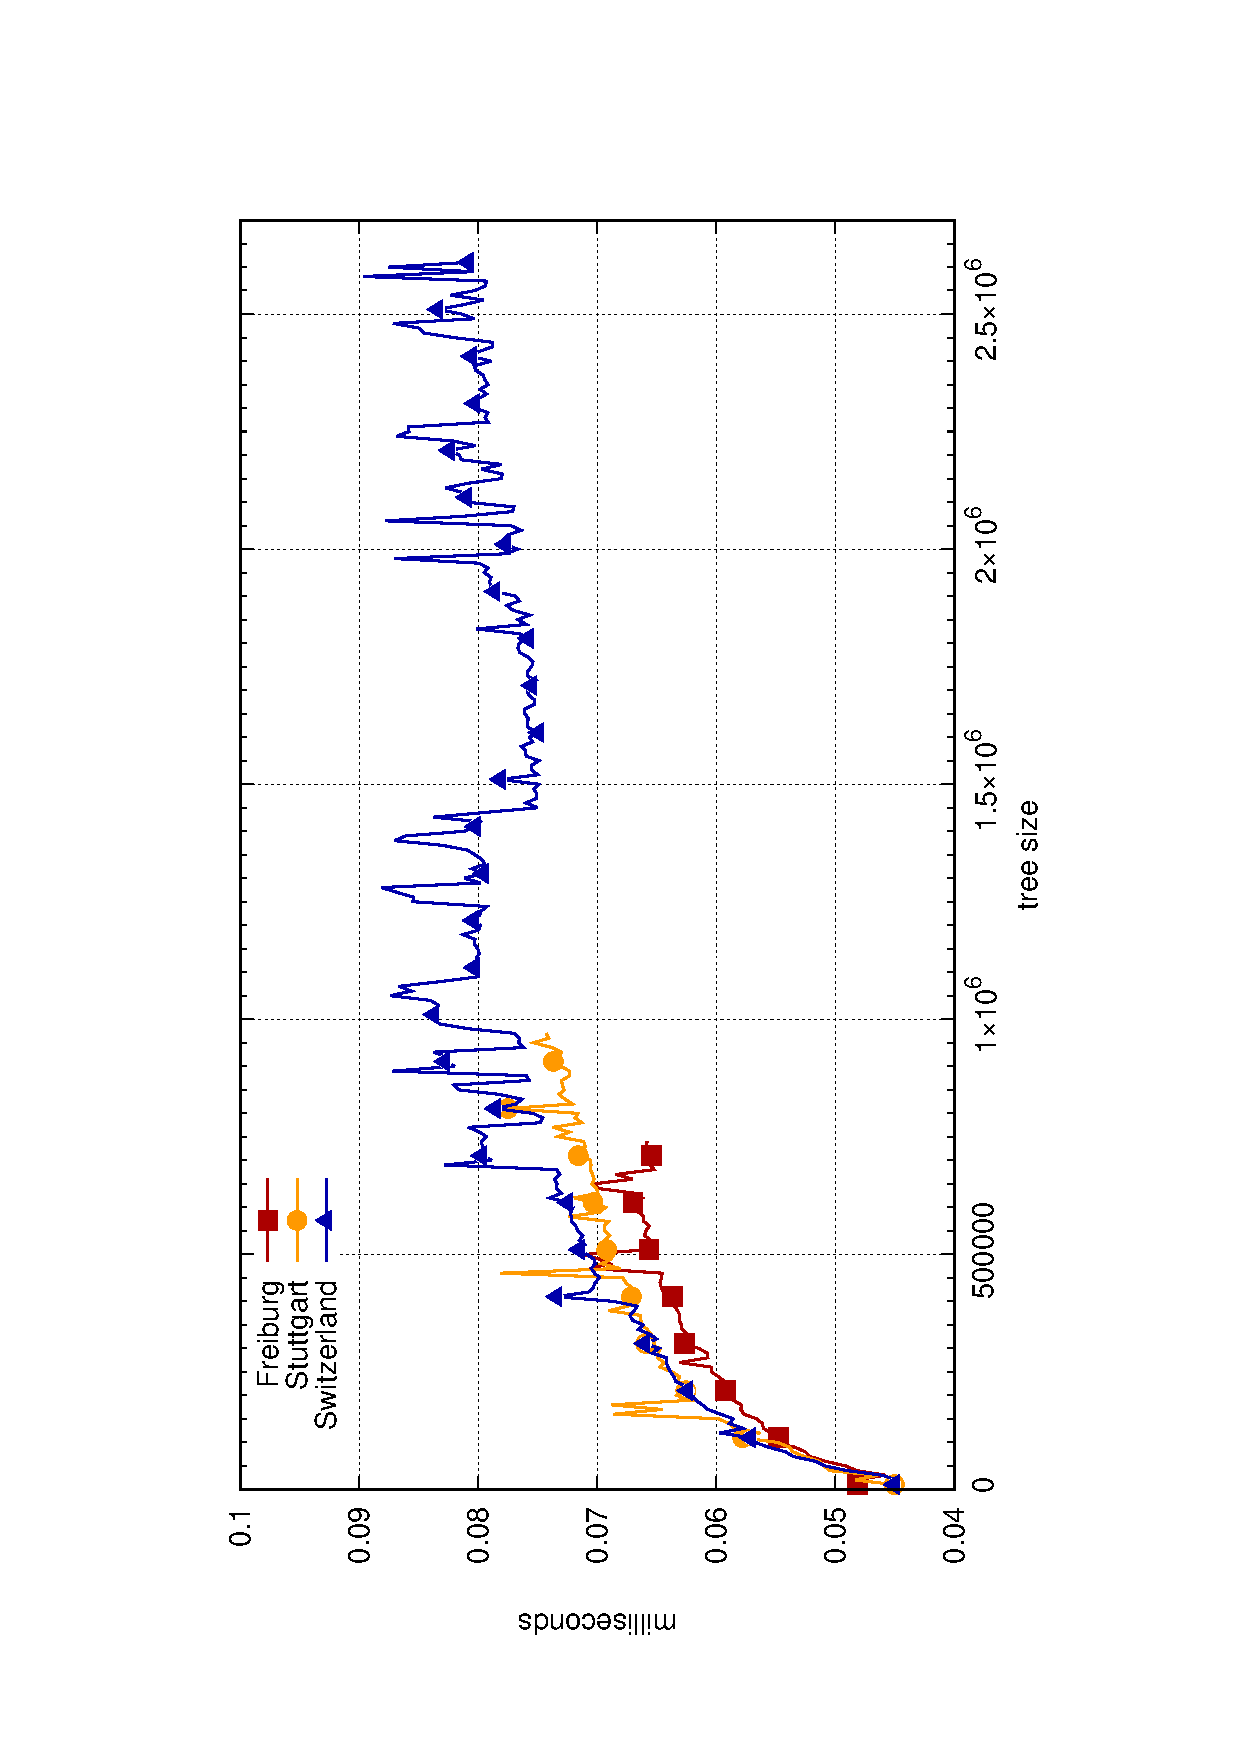
\includegraphics[scale=0.55,angle=-90]{res/plots/coverTreeResults}
		\end{center}
		\caption{Query durations for \algoref{coverTreeSearch} in a \coverTree with increasing size,
		for three road networks respectively. Measurements are done at a size of $1$, $10\,000$ and then in steps
		of $10\,000$, averaged over $1\,000$ random queries. Running time is stated in milliseconds.}
		\label{coverTreeResults}
	\end{figure}\quad\\
	\figref{coverTreeResults} shows the results of the experiment. The method is comparably fast, even for large road
	networks like \switzerlandR. The graph appears to be similar for all three data sets. This is obviously due to the fact that
	they all represent the same type of network, with a similar distribution of nodes.
	
	In a road network, nodes are typically close to each other and appear in local groups, representing cities and structured
	road segments. In particular, they are not uniformly distributed. A \coverTree benefits from this, as a node can be the
	parent of many other, locally close nodes. And as such, the tree is balanced well, resulting in efficient queries
	that are able to quickly find the correct path in the tree that leads to the nearest neighbor.
	
	Due to the same reason, the running time scales approximately logarithmic with increasing size. Queries take longer if the
	depth of the tree increases. In a well balanced \coverTree the depth is logarithmic to its size.

%Uni-modal routing
\subsection{Uni-modal routing}
	The first experiment for \uniModal routing compares time-independent methods for solving the \shortestPathProblem.
	It measures an implementation of \dijkstra (see \algoref{dijkstra}), the \astar algorithm (see \sectionref{alt})
	using $\asTheCrowFlies$ as heuristic and \alt with the precomputed heuristic shown in \defref{alt_heuristic}.
	
	Queries are performed on the road graphs obtained by the data sets \freiburgR, \stuttgartR and \switzerlandR.
	We choose $50$ random source nodes and then determine the \textit{Dijkstra rank} (see \defref{dijkstraRank})
	for the source nodes to all other nodes in the graph. Source nodes with a bad connectivity are rejected and exchanged
	against another random source node. This is determined by a source node having no node in the graph with a rank of at
	least $2^{15}$ which is only rarely the case for randomly chosen nodes.
	We then choose nodes as destinations that have a Dijkstra rank of
	\begin{align*}
		2^0, 2^1, \ldots, 2^k
	\end{align*}
	where $k \ge 15$ is the maximal rank all source nodes have in common. By that, the queries cover all types of
	ranges, highlighting how well the algorithms scale with queries of increasing ranges.
	By that, we receive for every rank $2^i$ in total $50$ different queries of which we average the
	measured running time over.\\
	% Uni-modal time-independent results
	\begin{figure}[!ht]
		 \begin{center}
			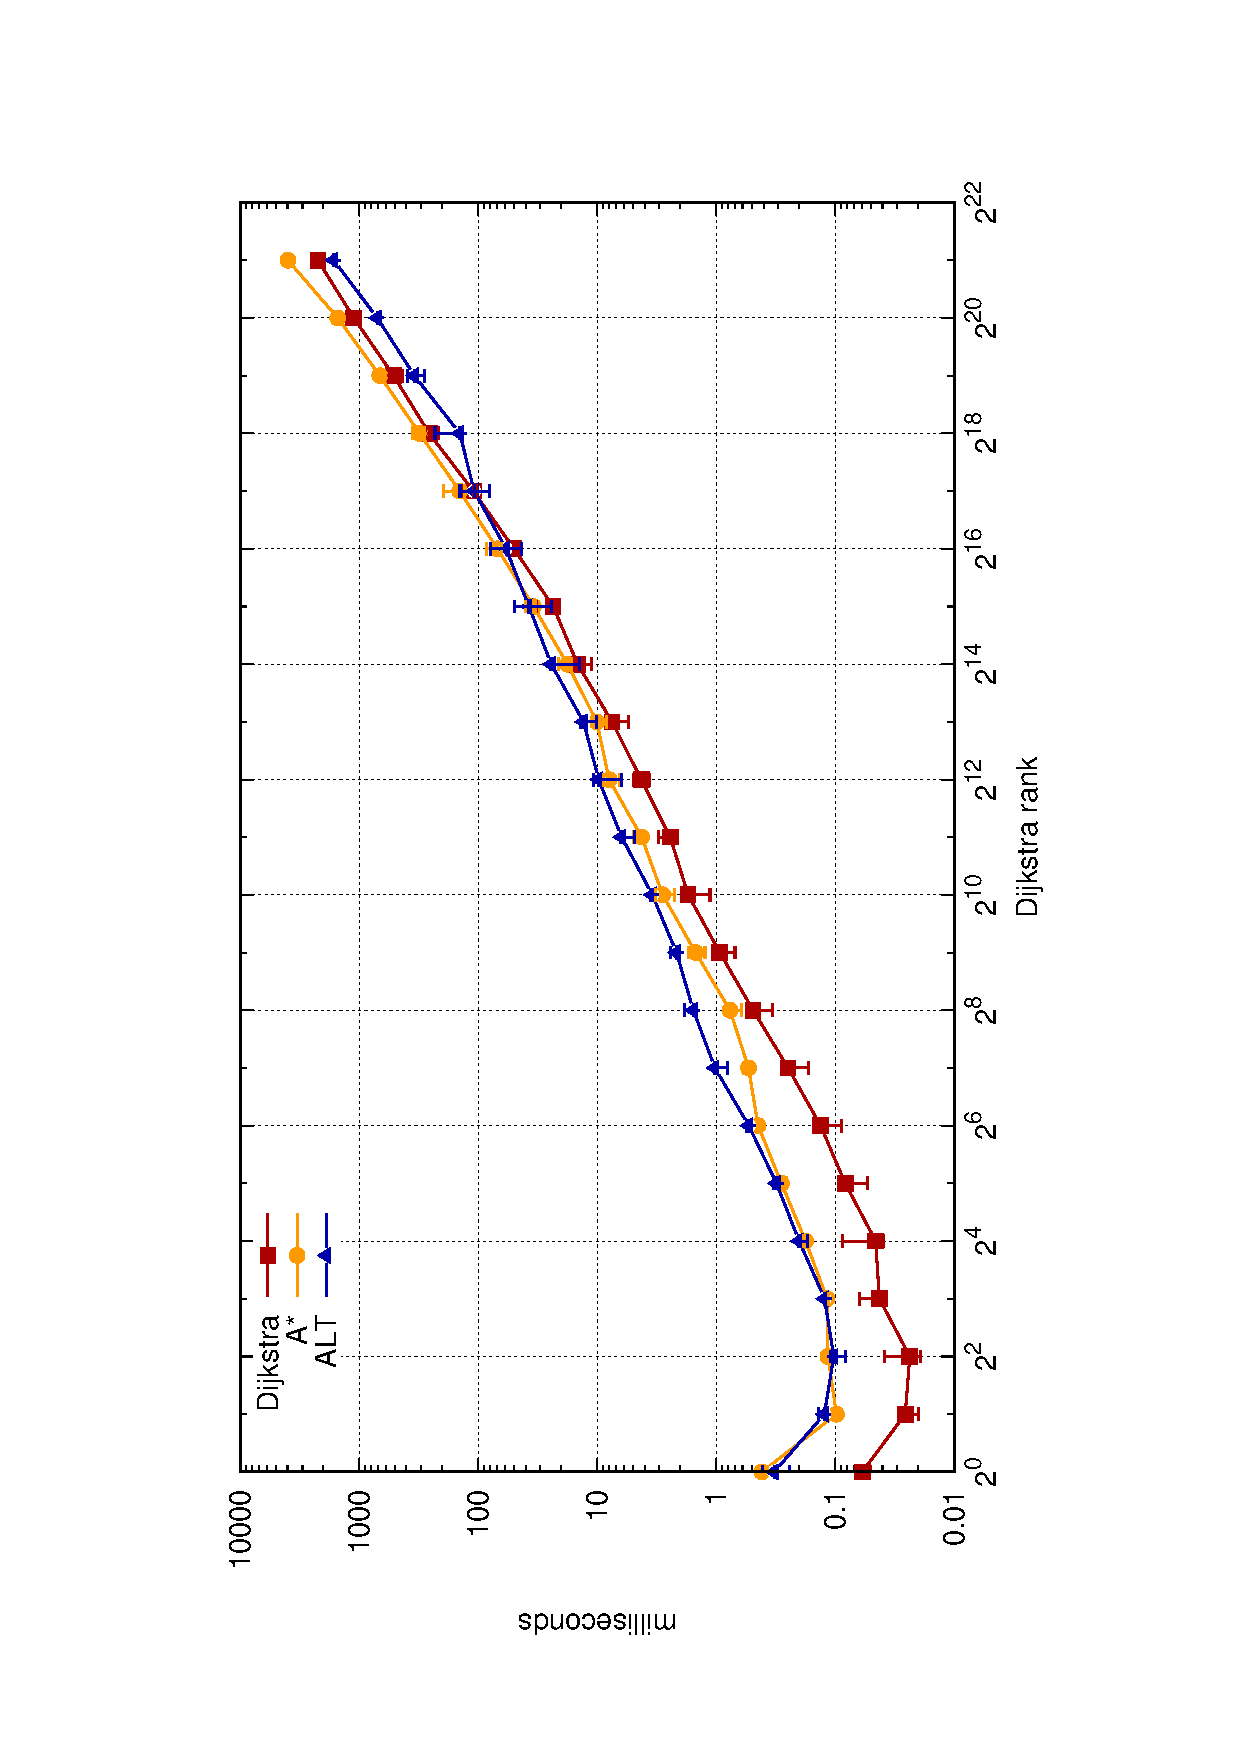
\includegraphics[scale=0.55,angle=-90]{res/plots/uniModalTimeIndependentResults}
		\end{center}
		\caption{Query durations for \uniModal time-independent route planning algorithms computing shortest paths.
			Running time is measured in milliseconds, presented on a logarithmic scale.
			Every point represents $50$ queries from a random source to a random target with the given \textit{Dijkstra rank}
			over which the measurement is averaged over. \textit{Errorbars} indicate the results on the three data sets.
			The upper end of the bar represents \switzerlandR, the dot \stuttgartR and the lower end \freiburgR.}
		\label{uniModalTimeIndependentResults}
	\end{figure}\quad\\
	\figref{uniModalTimeIndependentResults} shows the results of the experiment. First of all, it can be seen that all
	three methods do not scale well with queries of increasing ranges. Long range queries, like for a rank of $2^{20}$ or $2^{21}$ range
	from $1$ to $10$ seconds. In fact, the running time scales exponentially for increasing ranges. Further, \astar and \alt are slower
	than \dijkstra for short range queries. This is due to the increased overhead of the modified \dijkstra variants. Both need to
	additionally evaluate their corresponding heuristic on every relaxed edge. However, for mid and, in particular, for long
	range queries, \astar performs similar to \dijkstra and \alt even is about twice as fast. At this point the additional overhead is
	negligible and the benefit of a good heuristic pays off. It can also be seen that $\asTheCrowFlies$, which is used by \astar, is not a good
	heuristic for road networks and does not improve over the ordinary \dijkstra approach, as already explained in \sectionref{alt}.\\
	% Uni-modal time-independent results external
	\begin{figure}[!ht]
		 \begin{center}
			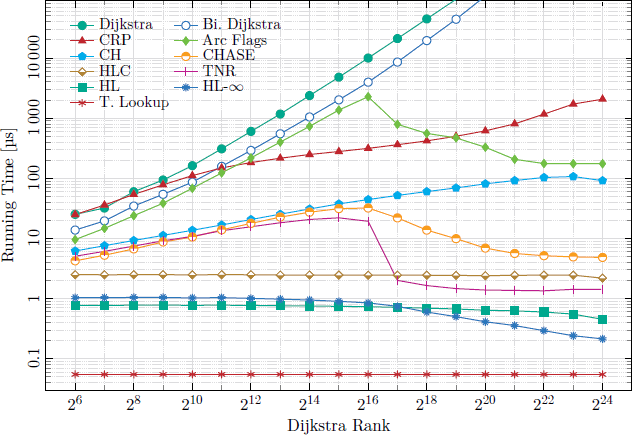
\includegraphics[scale=0.75]{res/uniModalTimeIndependentResultsExternal}
		\end{center}
		\caption{Experimental results from \libref{routePlanningOverview} measured similar to \figref{uniModalTimeIndependentResults}
			for carefully implemented \uniModal time-independent route planning algorithms.}
		\label{uniModalTimeIndependentResultsExternal}
	\end{figure}\quad\\
	Furthermore, if \alt is implemented very carefully and optimized, it can outperform \dijkstra earlier. For a comparison, we include the results
	from \libref{routePlanningOverview} of similar measured experiments for highly optimized variants of \dijkstra and other
	techniques for \uniModal time-independent route planning in \figref{uniModalTimeIndependentResultsExternal}.
	The results show that {\dijkstra}s performance can be increased by approximately a factor of $1\,000$, compared to our implementation,
	if heavily optimized. However, the running time for long range queries is still not feasible. Fortunately, there exist other approaches
	which tackle this problem, like seen in the figure. The presented algorithms are referenced and briefly explained in \libref{routePlanningOverview}.
	
	Additionally, they give a general overview of \uniModal time-independent route planning techniques, comparing their average query time and
	their necessary preprocessing time. We include their overview in \figref{uniModalTimeIndependentResultsExternalOverview}.\\
	% Uni-modal time-independent results external overview
	\begin{figure}[!ht]
		 \begin{center}
			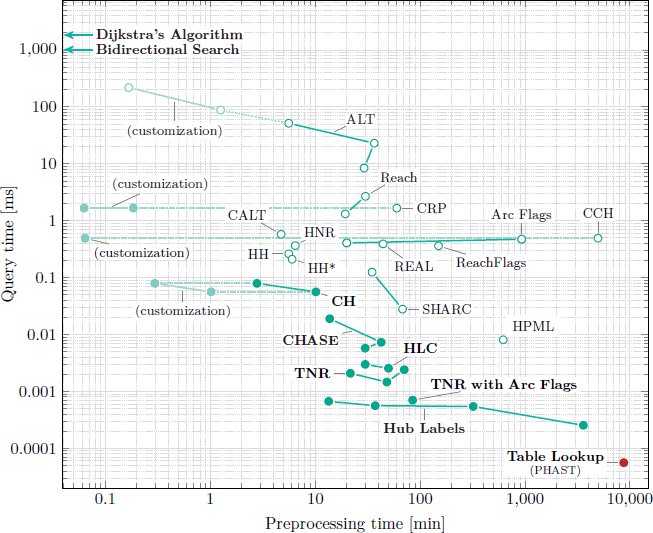
\includegraphics[scale=0.75]{res/uniModalTimeIndependentResultsExternalOverview}
		\end{center}
		\caption{Overview from \libref{routePlanningOverview} of \uniModal time-independent route planning
			techniques, comparing their average query time in milliseconds and their necessary preprocessing time in minutes.}
		\label{uniModalTimeIndependentResultsExternalOverview}
	\end{figure}\quad\\
	The second experiment compares time-dependent solutions to the \shortestPathProblem. We measure the performance of an
	adopted \dijkstra variant (see \sectionref{time_dependent_sec}) against \csa (using \algoref{csa_algo}) over the duration of one day,
	with changing time. The experiment is measured for the $10.10.2018$, which is a Wednesday, representing an average day in the schedule
	of the transit network. \dijkstra runs on a realistic time expanded transit graph (see \defref{realisticTransitGraph}) and \csa on a
	timetable (see \defref{timetable}), both obtained from the public transit data of \freiburgR, \stuttgartR and \switzerlandR.
	
	Measurements are taken in steps of $10$ minutes over the whole day, averaged over $50$ randomly chosen queries.
	The only exception is \dijkstra for \switzerlandR, which is done in steps of $30$ minutes, due to very long running times.\\
	 % Uni-modal time-dependent results all
	\begin{figure}[!ht]
		 \begin{center}
			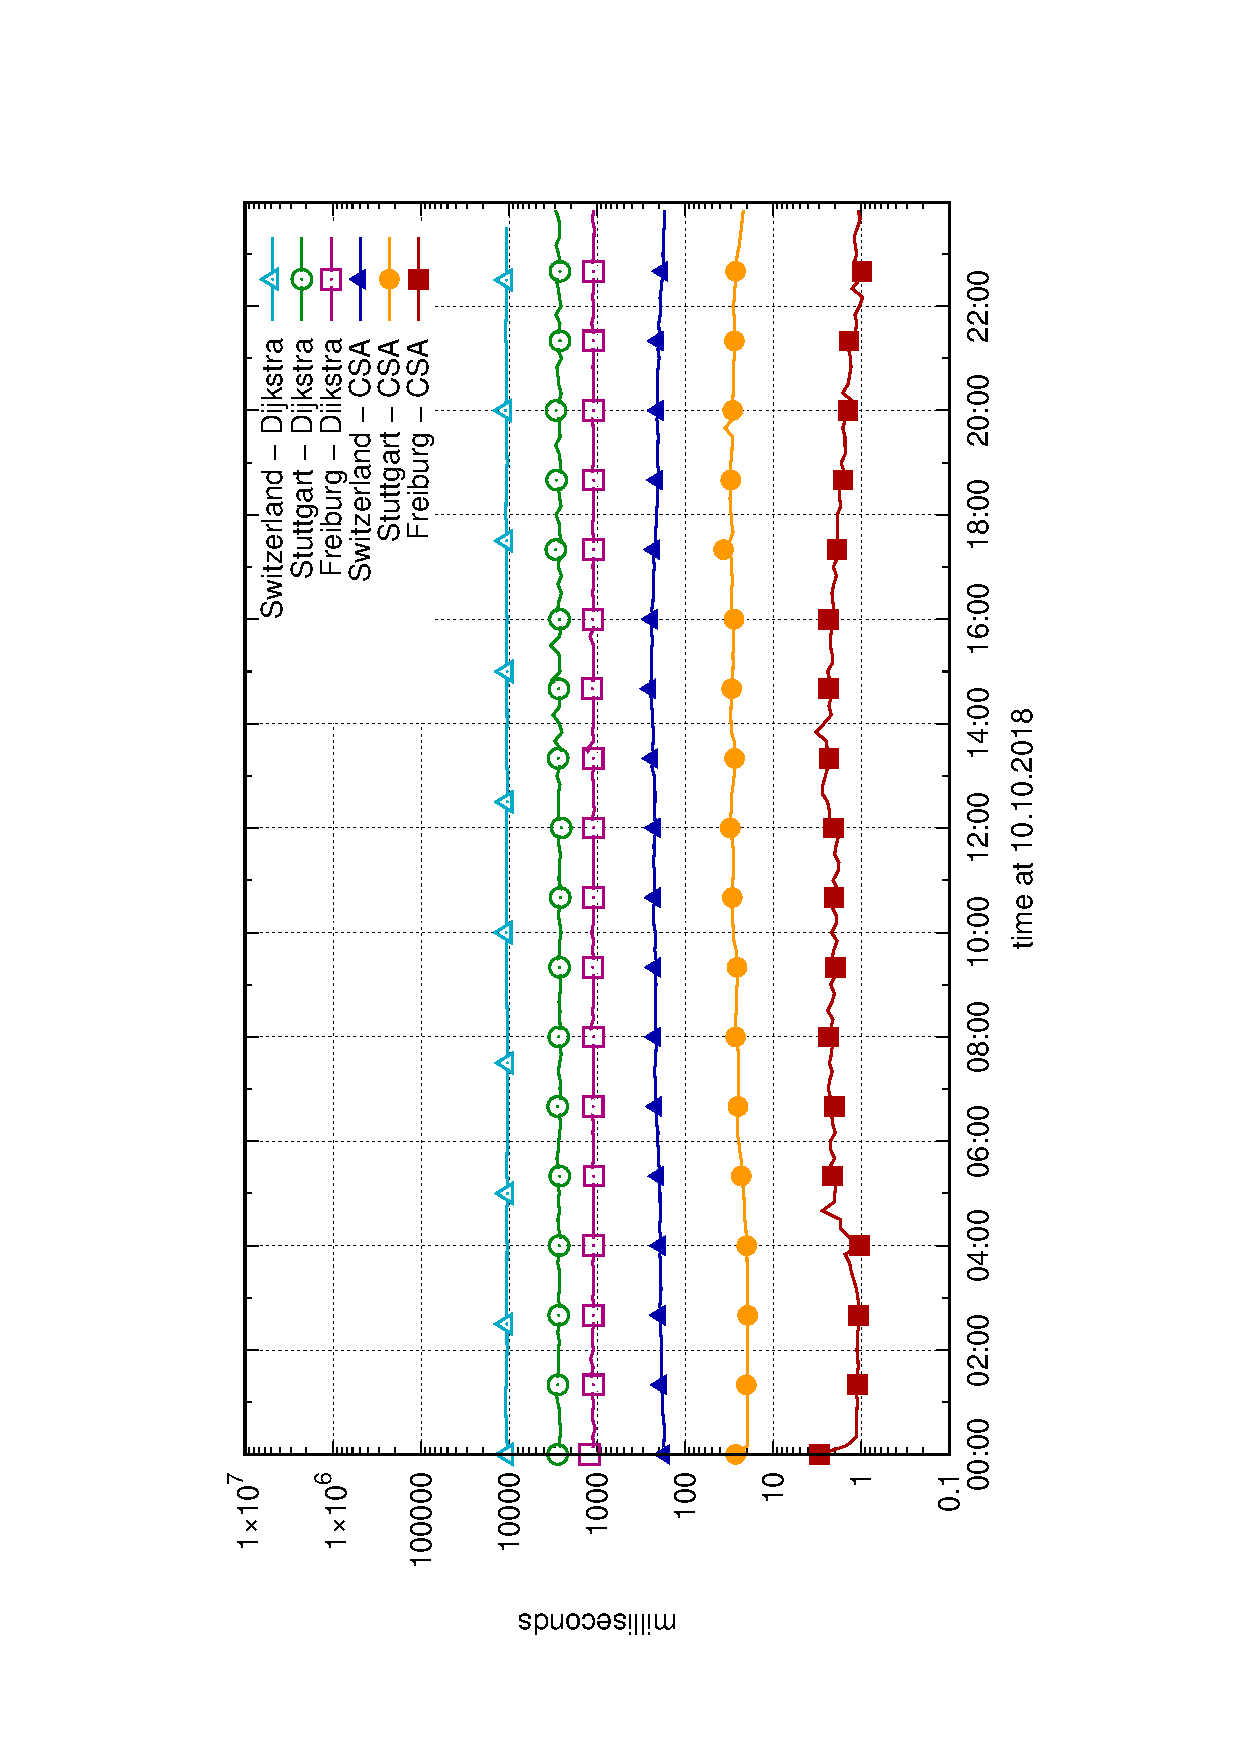
\includegraphics[scale=0.55,angle=-90]{res/plots/uniModalTimeDependentResultsAll}
		\end{center}
		\caption{Query durations of an time-independent variant of \dijkstra and \csa for three data sets, measured in milliseconds
			on a logarithmic scale. Measurements are done for every $10$ minutes of the $10.10.2018$, averaged over $50$ random queries.
			\dijkstra for \switzerlandR is measured in steps of $30$ minutes.}
		\label{uniModalTimeDependentResultsAll}
	\end{figure}
	% Uni-modal time-dependent results single
	\begin{figure}[!ht]
		 \begin{center}
			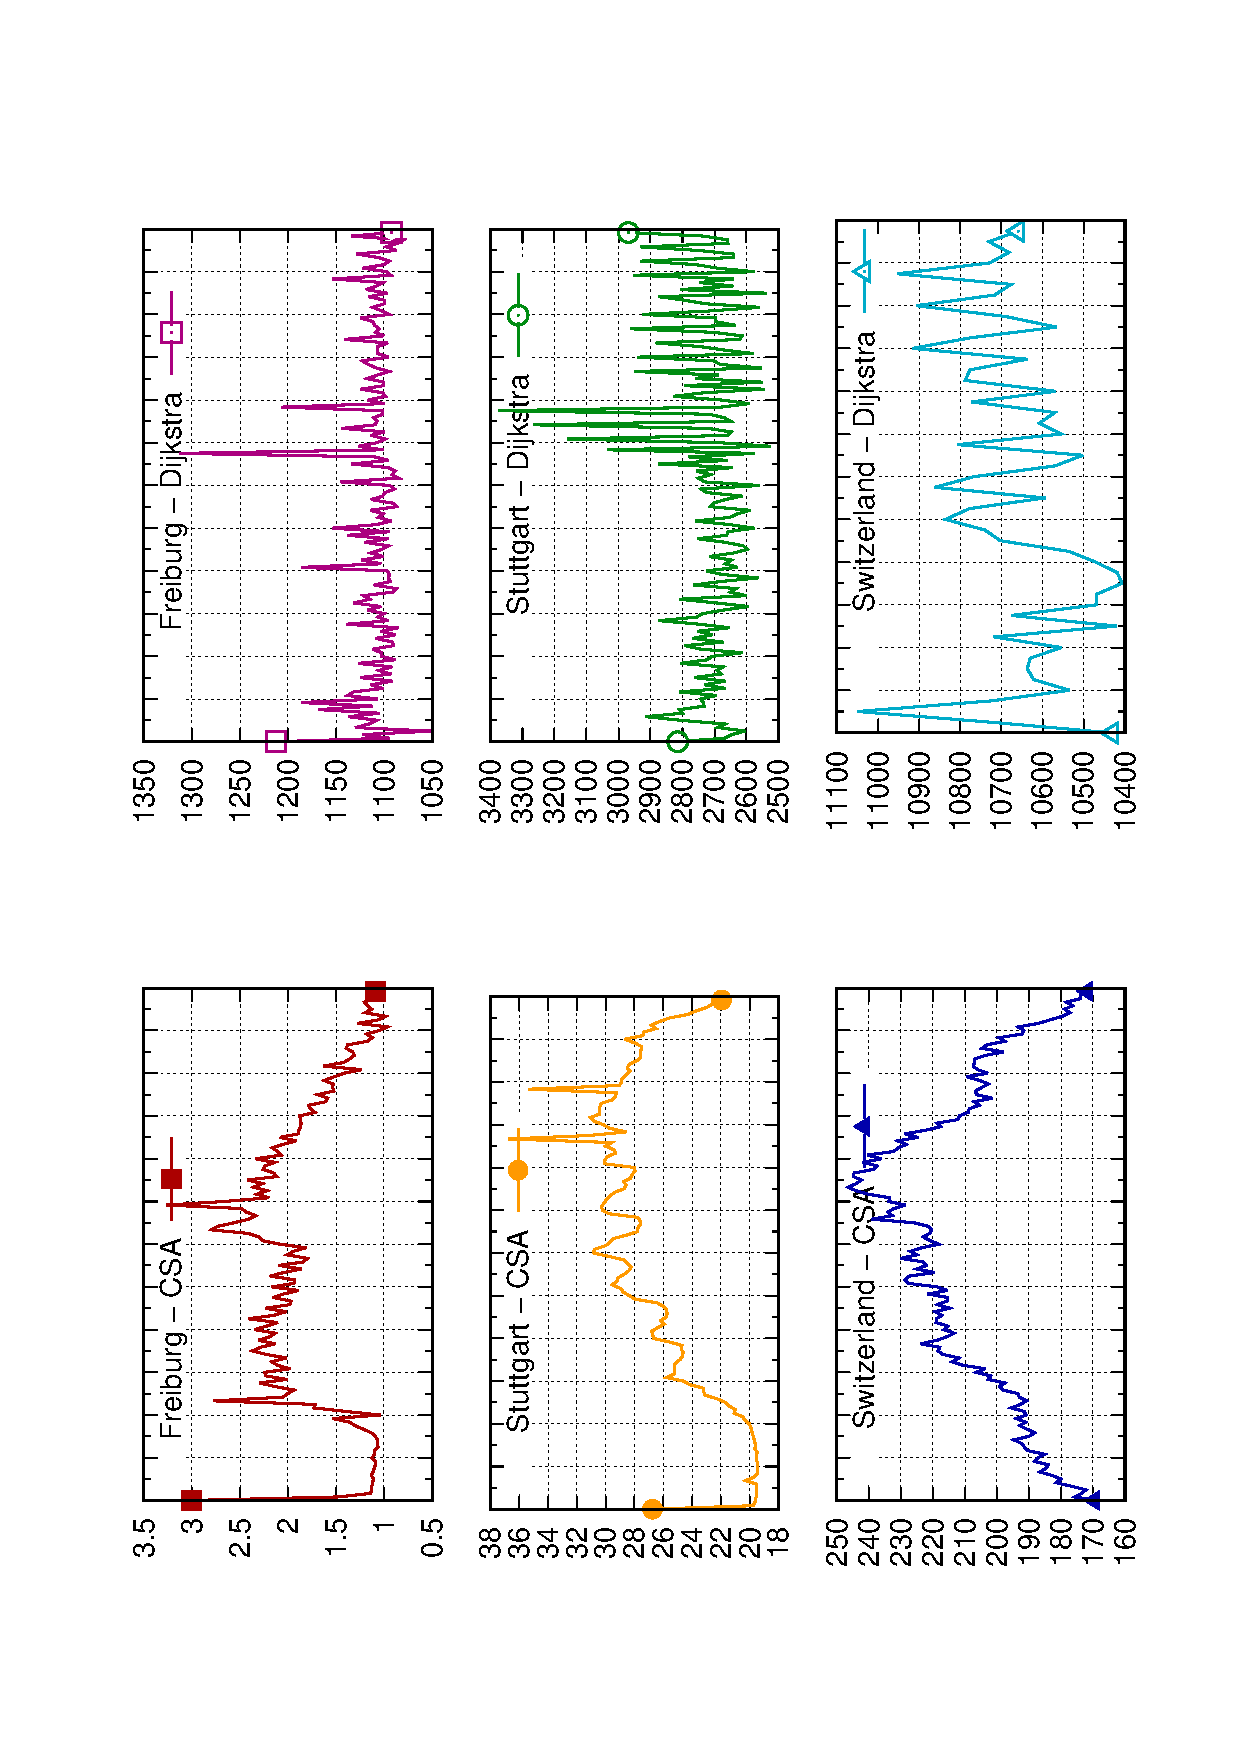
\includegraphics[scale=0.55,angle=-90]{res/plots/uniModalTimeDependentResultsSingle}
		\end{center}
		\caption{Results from \figref{uniModalTimeDependentResultsAll}, but isolated and with a linear scale for the query duration.
			The duration is measured in milliseconds and all graphs range from \timef{12}{00}{am} to \timef{11}{59}{pm} for the $10.10.2018$.}
		\label{uniModalTimeDependentResultsSingle}
	\end{figure}\quad\\
	 The algorithms are compared in \figref{uniModalTimeDependentResultsAll}, with their single performance
	 highlighted by \figref{uniModalTimeDependentResultsSingle}.
	 
	 Both algorithms perform worse if the size of the time schedule increases, roughly increasing by a factor of $10$ for all three data sets.
	 However, \csa runs on \switzerlandR $10$ times faster than \dijkstra on the small schedule of \freiburgR, where \csa even performs better
	 by a factor of $1\,000$. Clearly, \csa outperforms \dijkstra for time-dependent routing, making it a very viable choice. \csa can even successfully
	 compete against other approaches designed especially for time-dependent route planning, as shown by \libref{csa}.
	 
	 It can also be seen that \csa is subject to the traffic congestion of the time schedule. Yielding better running times in the evening and night
	 from \timef{6}{00}{pm} to \timef{6}{00}{am}, than in the morning, noon and afternoon from \timef{6}{00}{am} to \timef{6}{00}{pm}.
	 This is due to the fact that \csa needs to iterate all connections from a given time, not only relevant connections. In a rush hour, the schedule
	 has way more connections that need to be processed, leading to a worse performance.
	 
	 \dijkstra, on the other hand, only needs to scan connections available from the already processed routes. Thus, it is not affected by traffic
	 congestion as much as \csa and is still more subject to the range of queries, which is not captured by this experiment.

%Multi-modal routing
\subsection{Multi-modal routing}
	For \multiModal routing we compare a modified \dijkstra (see \sectionref{modifiedDijkstra}), running on a link graph (see \defref{linkGraph}), with
	our simplified version of \anr (refer to \sectionref{accessNodes}. \anr runs on a road graph and a timetable, using an ordinary \dijkstra for the road
	and \csa for the transit network. For a given query, it computes the three nearest neighbors to the source and destination as access nodes,
	using a \coverTree, then it runs \dijkstra to compute the shortest paths from the source and destination to their access nodes. After that, \csa is
	used to compute the shortest paths between the sources and destinations access nodes. Additionally, one shortest path query from the source
	to the destination, limited to the road network, is run. In total this makes
	\begin{itemize}
		\item[] $2 \times$ $3$-nearest neighbor queries from source and destination,
		\item[] $6 \times$ \dijkstra from source and destination to access nodes,
		\item[] $9 \times$ \csa between access nodes,
		\item[] $1 \times$ \dijkstra from source to destination, limited to the road graph.
	\end{itemize}
	The measurement is done similar to the experiments for \uniModal time-independent routing, as seen
	in \figref{uniModalTimeIndependentResults}, measuring for specific increasing \textit{Dikstra rank}s. Additionally, the measurement is fixed
	to the $10.10.2018$ at \timef{12}{00}{pm}. The first experiment has no limitations on the transportation modes. All modes of the set
	\begin{align*}
		\{\car, \bike, \foot, \tram\}
	\end{align*}
	are available, while the second experiment limits the available modes to
	\begin{align*}
		\{\bike, \tram\}.
	\end{align*}
	The results are given by \figref{multiModalResultsBaseline} and \figref{multiModalResultsRestricted} respectively.\\
	% Multi-modal results baseline
	\begin{figure}[!ht]
		 \begin{center}
			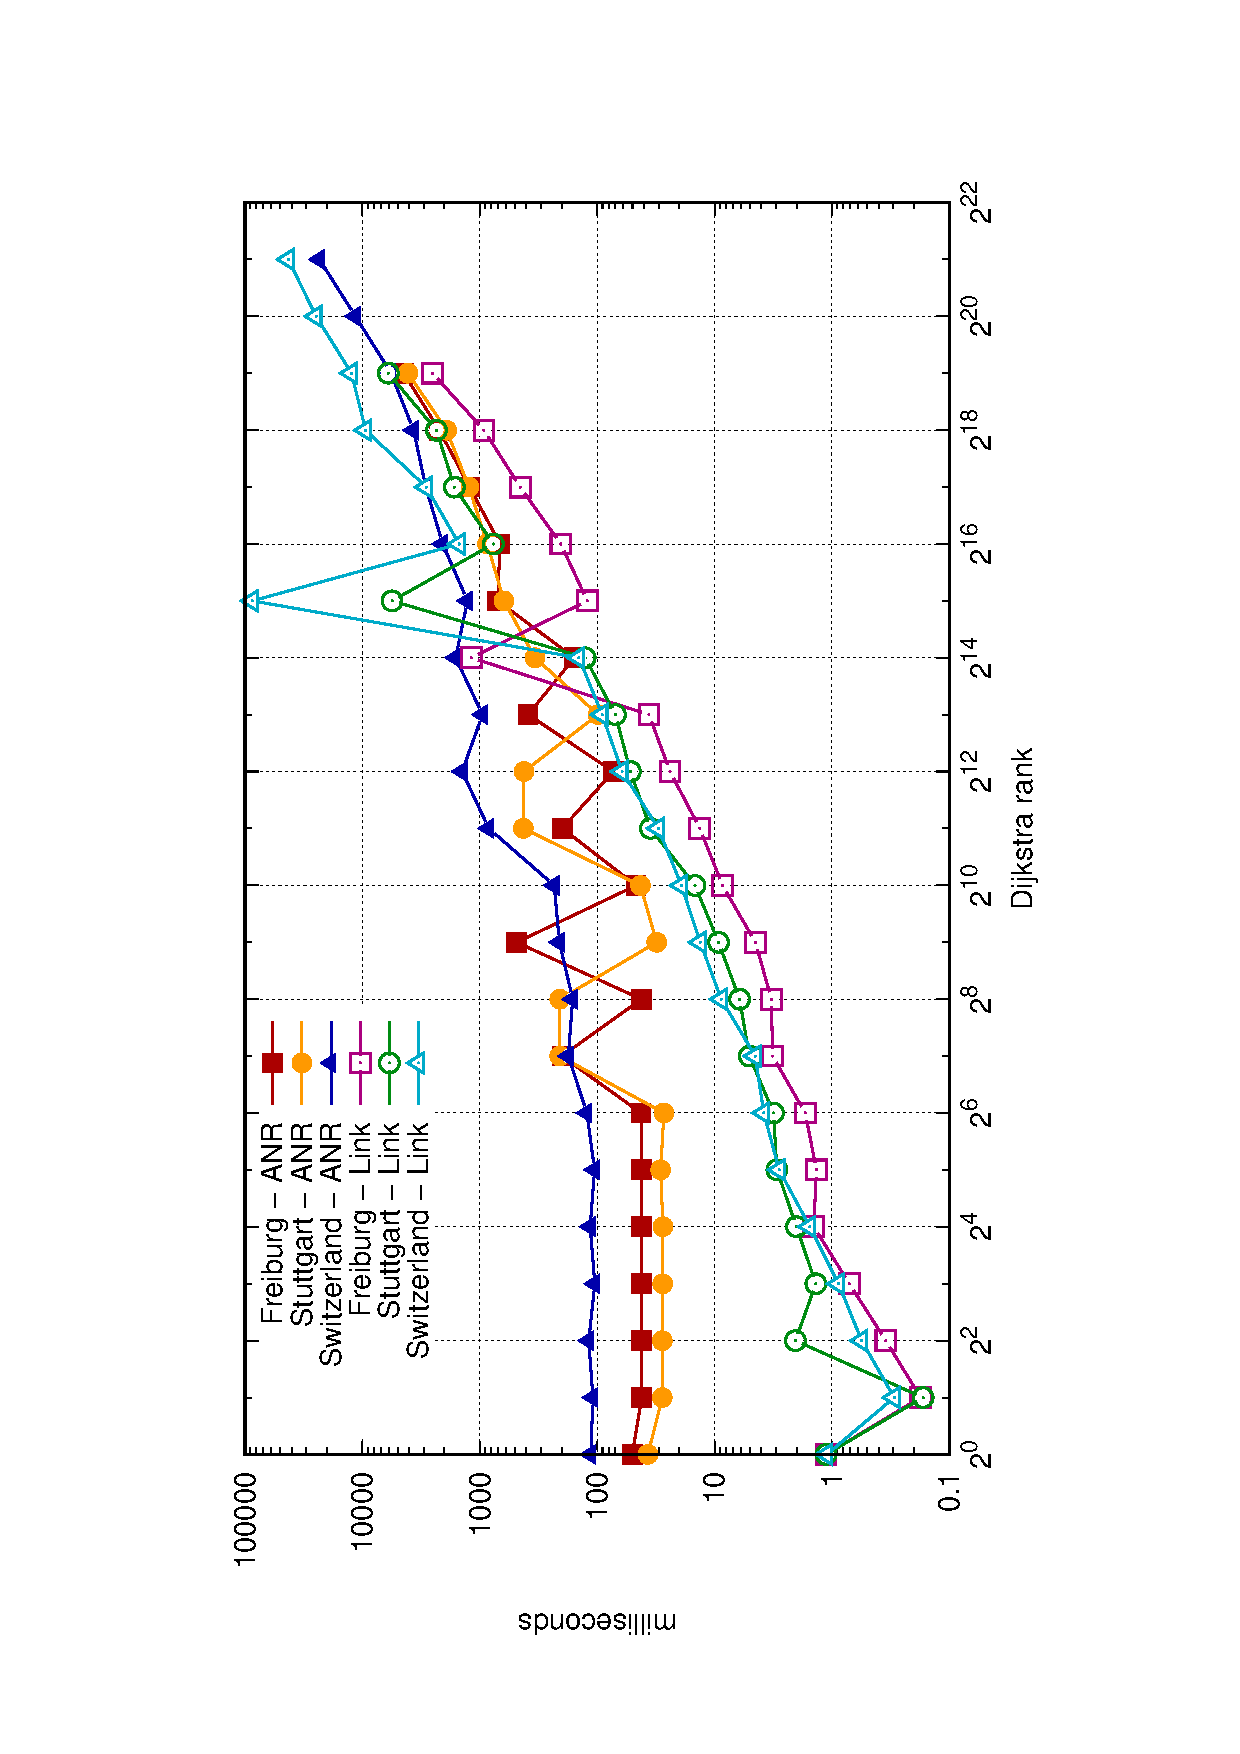
\includegraphics[scale=0.55,angle=-90]{res/plots/multiModalResultsBaseline}
		\end{center}
		\caption{Results of \multiModal route planning with transportation modes $\{\car, \bike, \foot, \tram\}$.
			Query duration of \dijkstra on a link graph and a simplified version of \anr using \dijkstra on a road graph and \csa on a timetable
			are shown. Measurements are averaged over $50$ random queries with the specified Dijkstra rank. Query duration is measured
			in milliseconds, presented on a logarithmic scale.}
		\label{multiModalResultsBaseline}
	\end{figure}
	% Multi-modal results restricted
	\begin{figure}[!ht]
		 \begin{center}
			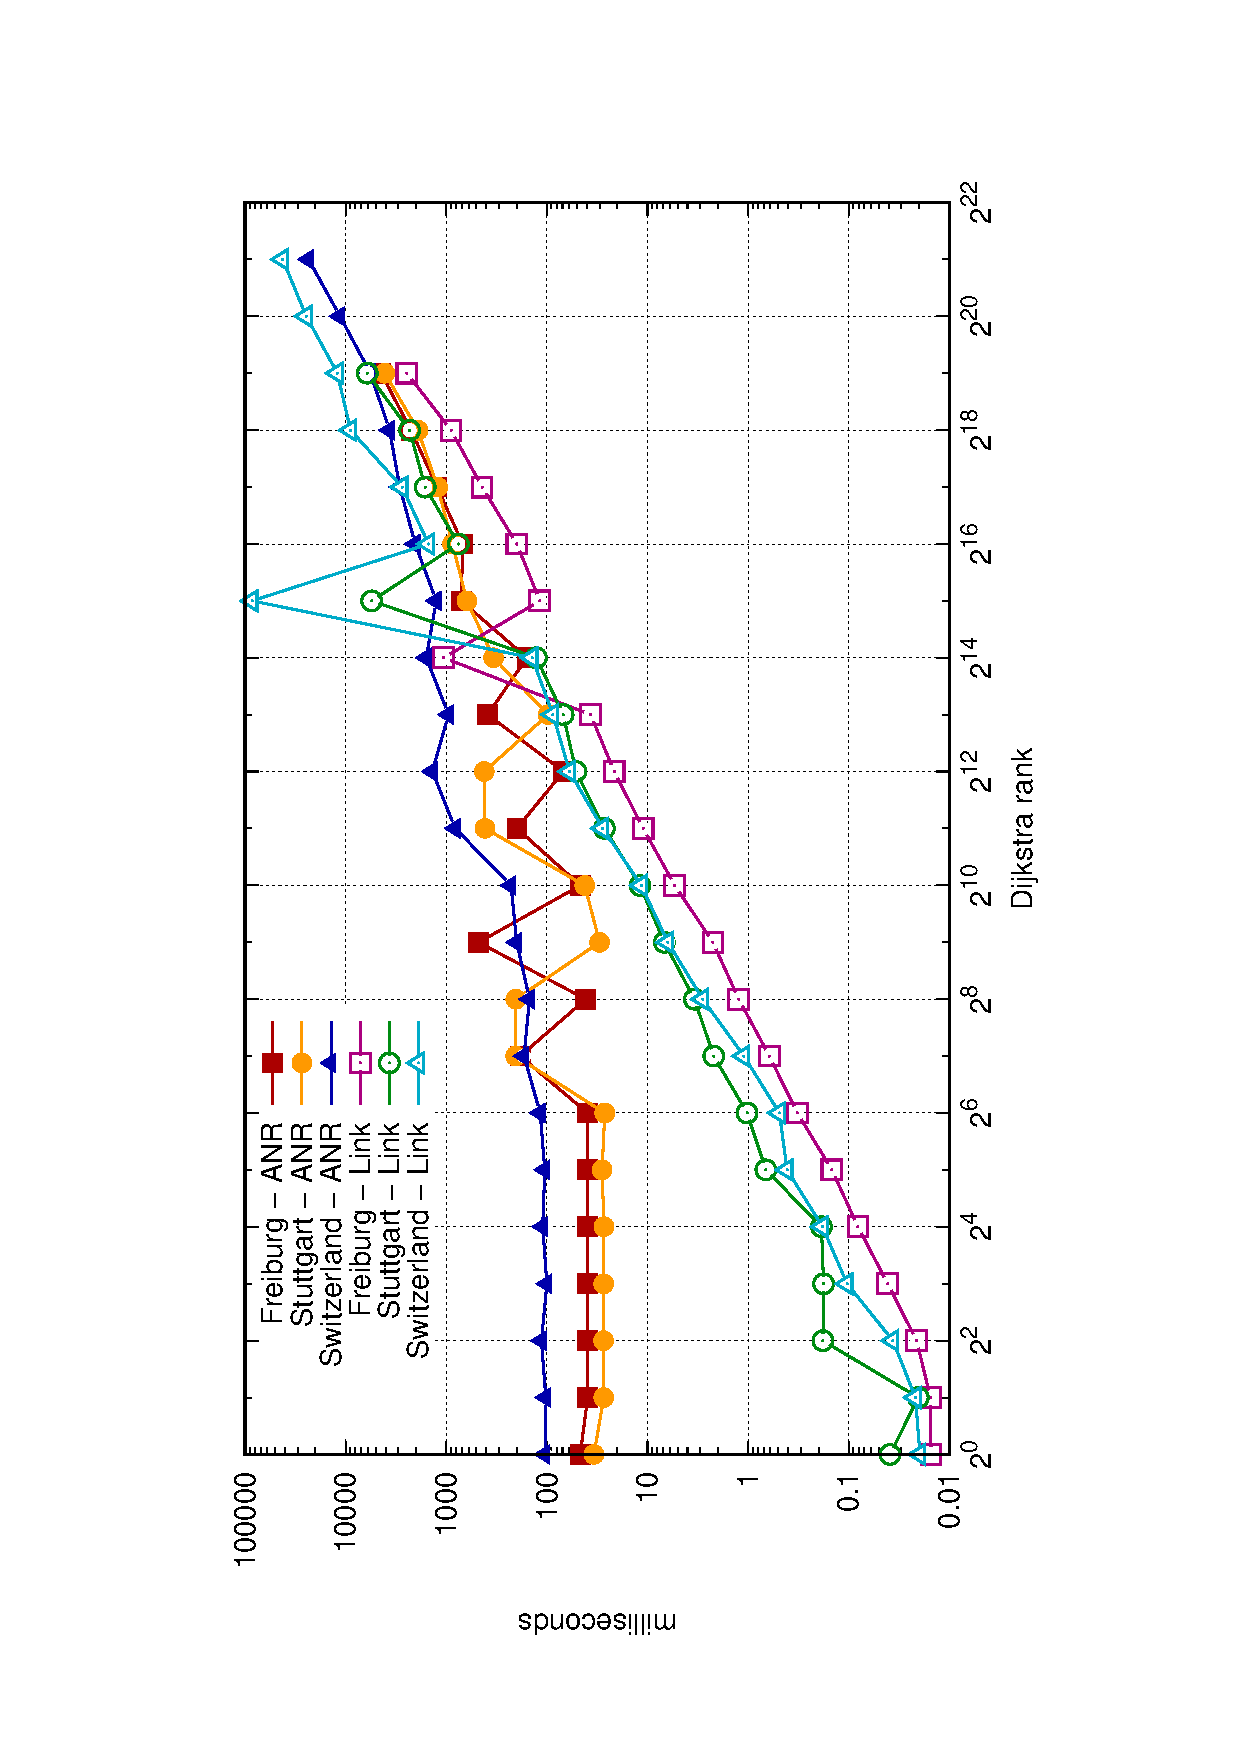
\includegraphics[scale=0.55,angle=-90]{res/plots/multiModalResultsRestricted}
		\end{center}
		\caption{Experiment from \figref{multiModalResultsBaseline}, but restricted to the transportation modes $\{\bike, \tram\}$.}
		\label{multiModalResultsRestricted}
	\end{figure}\quad\\
	Transportation mode restrictions do not impair the running time of \dijkstra or \anr. Which is due to \dijkstra not using any
	optimizations relying on transportation modes. Computation is done on the fly, without using precomputed results. The same holds for
	the simplified \anr, which uses ordinary \dijkstra and \csa. Unfortunately, optimizations like \alt do not adapt well to \multiModal route planning,
	since the precomputation must be done under the assumption of specific transportation modes restrictions, which might be different at query time.
	
	A key problem of \dijkstra on link graphs is that its running time is not applicable for long range queries and that a link graph scales
	very bad in space consumption. In our experiments, the link graph for \switzerlandR consumes approximately $75$ GB, while \anr allocates
	only about $15$ GB for the road graph and the timetable.\\\\
	As expected, the simplified version of \anr does not beat the ordinary \dijkstra, as it still needs to compute long range routes on the road graph
	using \dijkstra. The key problem of our approach is that access nodes, which are chosen as nearest neighbors, might be far away or not even
	be reachable when using the road network. Geographic proximity does not necessarily imply short travel times.
	In this case, the $6$ short range \dijkstra computations are actually long range computations, for which \dijkstra scales bad.
	
	However, \anr has one major advantage over \dijkstra. It can use any algorithm that computes shortest paths on a road network.
	This stands in contrast to the link graph approach which needs an algorithm that is able to route on a combined network, containing
	road and transit data. Because of that, a well implemented \anr uses a fast algorithm for road networks
	(compare to \figref{uniModalTimeIndependentResultsExternalOverview}) and selects access nodes more sophisticated. Which leads
	to \anr easily beating the query time of \dijkstra on link graphs, making it a feasible approach for \multiModal route planning
	(see \libref{accessNodeRouting}).